% Chapter 15. Four layers, and only the top one needs a model.
\documentclass[tikz,border=6pt]{standalone}
% Shared look for every TikZ figure in the book.
% Colours match book/preamble.tex exactly. Change both or neither.

\usepackage{tikz}
\usepackage{xcolor}
\usepackage{amsmath}
\IfFileExists{libertinus.sty}{\usepackage[mono=false]{libertinus}}{}
\IfFileExists{inconsolata.sty}{\usepackage[varqu,varl,scaled=0.95]{inconsolata}}{}

\usetikzlibrary{
  arrows.meta, positioning, calc, fit, backgrounds, shapes.geometric,
  shapes.misc, decorations.pathreplacing, decorations.pathmorphing,
  patterns, chains, matrix, shadows.blur
}

\definecolor{ink}{HTML}{15181D}
\definecolor{muted}{HTML}{5B6472}
\definecolor{rule}{HTML}{C9CED6}
\definecolor{wash}{HTML}{F4F5F7}
\definecolor{accent}{HTML}{0F5C8C}
\definecolor{accentsoft}{HTML}{E7F0F6}
\definecolor{warm}{HTML}{B4531A}
\definecolor{warmsoft}{HTML}{FBF0E7}
\definecolor{good}{HTML}{2C6E49}
\definecolor{goodsoft}{HTML}{E9F2EC}
\definecolor{danger}{HTML}{9B2226}
\definecolor{dangersoft}{HTML}{FAECEC}

\tikzset{
  font=\sffamily\small,
  >={Stealth[length=5pt, width=4pt]},
  %
  box/.style={
    draw=rule, line width=0.8pt, fill=wash, rounded corners=2pt,
    inner sep=7pt, align=center, text=ink, minimum height=9mm,
  },
  boxa/.style={box, draw=accent, fill=accentsoft},
  boxg/.style={box, draw=good,   fill=goodsoft},
  boxw/.style={box, draw=warm,   fill=warmsoft},
  boxd/.style={box, draw=danger, fill=dangersoft},
  %
  lane/.style={draw=rule, line width=0.7pt, fill=white, rounded corners=2pt,
               inner sep=6pt, align=center, minimum width=26mm},
  %
  flow/.style={draw=accent, line width=1.0pt, ->},
  flowback/.style={flow, densely dashed},
  flowmuted/.style={draw=muted, line width=0.8pt, ->},
  lifeline/.style={draw=rule, line width=0.7pt, densely dotted},
  %
  lbl/.style={font=\sffamily\scriptsize, text=muted, inner sep=2pt},
  lblink/.style={font=\sffamily\scriptsize, text=ink, inner sep=2pt},
  tag/.style={font=\ttfamily\scriptsize, text=accent, inner sep=2pt,
              fill=white, inner xsep=3pt},
  note/.style={font=\sffamily\scriptsize\itshape, text=muted, align=left},
  %
  band/.style={draw=none, rounded corners=1pt},
  tick/.style={draw=muted, line width=0.6pt},
}

% A horizontal timeline bar segment: \barseg{x0}{x1}{y}{colour}{label}
\newcommand{\barseg}[5]{%
  \fill[#4, rounded corners=1pt] (#1,#3-0.16) rectangle (#2,#3+0.16);
  \node[lbl, text=white, font=\sffamily\scriptsize\bfseries]
       at ({(#1+#2)/2},#3) {#5};
}

\begin{document}
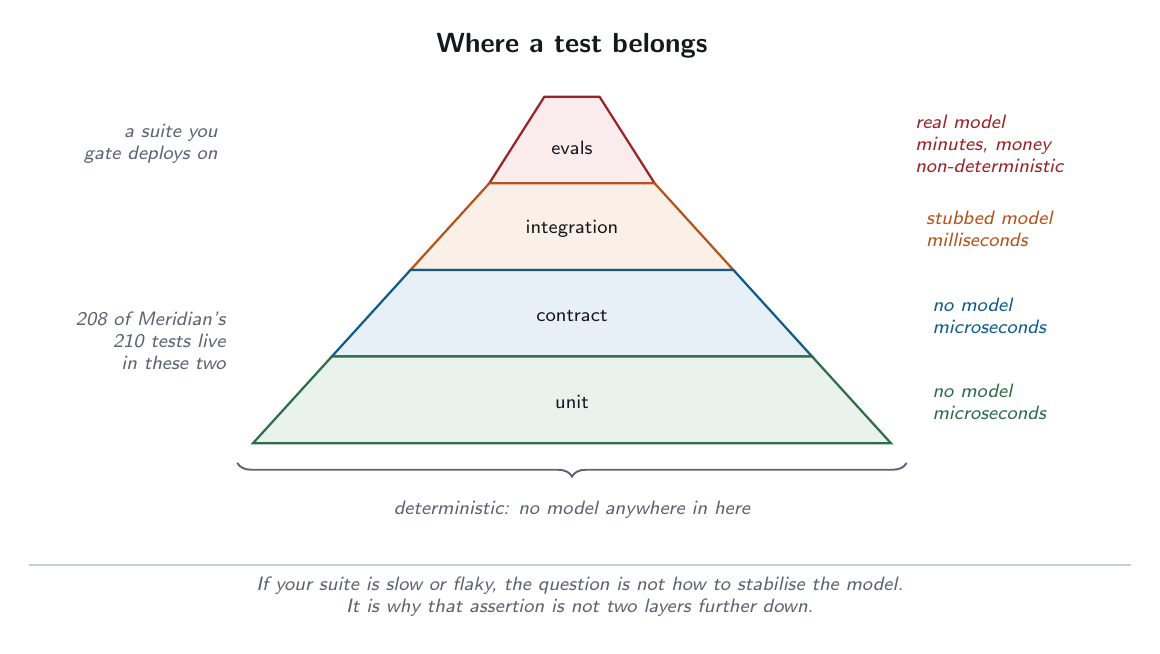
\begin{tikzpicture}[x=1cm, y=1cm]

  \node[lblink, font=\sffamily\bfseries] at (4.6,4.75) {Where a test belongs};

  \fill[dangersoft, draw=danger, line width=0.8pt]
    (3.55,3.0) -- (5.65,3.0) -- (4.95,4.1) -- (4.25,4.1) -- cycle;
  \node[font=\sffamily\scriptsize, text=ink] at (4.6,3.45) {evals};

  \fill[warmsoft, draw=warm, line width=0.8pt]
    (2.55,1.9) -- (6.65,1.9) -- (5.65,3.0) -- (3.55,3.0) -- cycle;
  \node[font=\sffamily\scriptsize, text=ink] at (4.6,2.42) {integration};

  \fill[accentsoft, draw=accent, line width=0.8pt]
    (1.55,0.8) -- (7.65,0.8) -- (6.65,1.9) -- (2.55,1.9) -- cycle;
  \node[font=\sffamily\scriptsize, text=ink] at (4.6,1.32) {contract};

  \fill[goodsoft, draw=good, line width=0.8pt]
    (0.55,-0.3) -- (8.65,-0.3) -- (7.65,0.8) -- (1.55,0.8) -- cycle;
  \node[font=\sffamily\scriptsize, text=ink] at (4.6,0.22) {unit};

  % right-hand annotations
  \node[note, align=left, text=danger] at (9.9,3.5)  {real model\\minutes, money\\non-deterministic};
  \node[note, align=left, text=warm]   at (9.9,2.42) {stubbed model\\milliseconds};
  \node[note, align=left, text=accent] at (9.9,1.32) {no model\\microseconds};
  \node[note, align=left, text=good]   at (9.9,0.22) {no model\\microseconds};

  % left-hand counts
  \node[note, align=right] at (-0.75,3.5)  {a suite you\\gate deploys on};
  \node[note, align=right] at (-0.75,1.0)  {208 of Meridian's\\210 tests live\\in these two};

  \draw[decorate, decoration={brace, amplitude=5pt, mirror}, draw=muted, line width=0.7pt]
    (0.35,-0.55) -- (8.85,-0.55);
  \node[note, align=center, text=muted] at (4.6,-1.15)
    {deterministic: no model anywhere in here};

  \draw[rule, line width=0.7pt] (-2.3,-1.85) -- (11.7,-1.85);
  \node[note, align=center, text=muted] at (4.7,-2.25)
    {If your suite is slow or flaky, the question is not how to stabilise the
     model.\\It is why that assertion is not two layers further down.};

\end{tikzpicture}
\end{document}
